\documentclass{standalone}
\usepackage{tikz}
%\usetikzlibrary{...}
\begin{document}
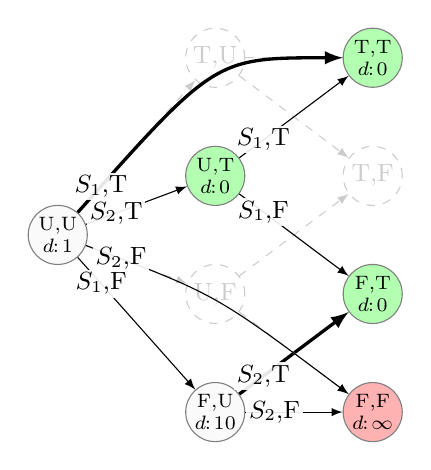
\begin{tikzpicture}[font=\small]

\tikzset{>=latex} % arrow heads

\node[draw=black!50,circle,inner sep=1pt,fill=black!2,minimum width=0.75cm,inner sep=0pt,align=center,font=\scriptsize] (uu) at (0,0) {U,U\\$d\!\!:\!1$};

\node[draw=black!50,circle,inner sep=1pt,fill=black!2,minimum width=0.75cm,inner sep=0pt,align=center,font=\scriptsize] (fu) at (2,-2.25) {F,U\\$d\!\!:\!10$};
\node[draw=black!20,dashed,circle,inner sep=1pt,minimum width=0.75cm,color=black!20] (uf) at (2,-0.75) {U,F};
\node[draw=black!50,circle,inner sep=1pt,fill=green!30,minimum width=0.75cm,inner sep=0pt,align=center,font=\scriptsize] (ut) at (2, 0.75) {U,T\\$d\!\!:\!0$};
\node[draw=black!20,dashed,circle,inner sep=1pt,minimum width=0.75cm,color=black!20] (tu) at (2, 2.25) {T,U};3
\node[draw=black!50,circle,inner sep=1pt,fill=red!30,minimum width=0.75cm,inner sep=0pt,align=center,font=\scriptsize] (ff) at (4,-2.25) {F,F\\$d\!\!:\!\infty$};
\node[draw=black!50,circle,inner sep=1pt,fill=green!30,minimum width=0.75cm,inner sep=0pt,align=center,font=\scriptsize] (ft) at (4,-0.75) {F,T\\$d\!\!:\!0$};
\node[draw=black!20,dashed,circle,inner sep=1pt,minimum width=0.75cm,color=black!20] (tf) at (4, 0.75) {T,F};
\node[draw=black!50,circle,inner sep=1pt,fill=green!30,minimum width=0.75cm,inner sep=0pt,align=center,font=\scriptsize] (tt) at (4, 2.25) {T,T\\$d\!\!:\!0$};

\draw[->] (uu) -- (fu) node[pos=0.20,inner sep=1pt,fill=white,fill opacity=0.9,text opacity=1.0] {$S_1$,F};
\draw[->,black!20,dashed] (uu) -- (tu);
\draw[->,black!20,dashed] (uu) -- (uf);
\draw[->] (uu) -- (ut) node[pos=0.30,inner sep=1pt,fill=white,fill opacity=0.9,text opacity=1.0] {$S_2$,T};

\draw[->] (fu) -- (ff) node[pos=0.30,inner sep=1pt,fill=white,fill opacity=0.9,text opacity=1.0] {$S_2$,F};
\draw[->,very thick] (fu) -- (ft) node[pos=0.22,inner sep=1pt,fill=white,fill opacity=0.9,text opacity=1.0] {$S_2$,T};

\draw[->,black!20,dashed] (tu) -- (tf);
\draw[->,black!20,dashed] (tu) -- (tt);

\draw[->,black!20,dashed] (uf) -- (ff);
\draw[->,black!20,dashed] (uf) -- (tf);

\draw[->] (ut) -- (ft) node[pos=0.22,inner sep=1pt,fill=white,fill opacity=0.9,text opacity=1.0] {$S_1$,F};
\draw[->] (ut) -- (tt) node[pos=0.22,inner sep=1pt,fill=white,fill opacity=0.9,text opacity=1.0] {$S_1$,T};

\draw[->,very thick] (uu) .. controls (tu) .. (tt) node[pos=0.06,inner sep=1pt,fill=white,fill opacity=0.9,text opacity=1.0] {$S_1$,T};
\draw[->] (uu) .. controls (uf) .. (ff) node[pos=0.10,inner sep=1pt,fill=white,fill opacity=0.9,text opacity=1.0] {$S_2$,F};


\end{tikzpicture}%
\end{document}
